% This is samplepaper.tex, a sample chapter demonstrating the
% LLNCS macro package for Springer Computer Science proceedings;
% Version 2.20 of 2017/10/04
%
\documentclass[runningheads]{llncs}
%
\usepackage{graphicx}
% Used for displaying a sample figure. If possible, figure files should
% be included in EPS format.
%
% If you use the hyperref package, please uncomment the following line
% to display URLs in blue roman font according to Springer's eBook style:
% \renewcommand\UrlFont{\color{blue}\rmfamily}

\begin{document}
%
\title{Transactions Fraud Detection using Machine Learning and Nature Inspired Algorithms}
%
%\titlerunning{Abbreviated paper title}
% If the paper title is too long for the running head, you can set
% an abbreviated paper title here
%
\author{Peter Mačinec \and Timotej Zaťko}
%
\authorrunning{Peter Mačinec, Timotej Zaťko}
% First names are abbreviated in the running head.
% If there are more than two authors, 'et al.' is used.
%
\institute{Faculty of Informatics and Information Technologies,\\Slovak University of Technology, Bratislava}
%
\maketitle              % typeset the header of the contribution
%
\begin{abstract}
The abstract should briefly summarize the contents of the paper in
15--250 words.

\keywords{Transactions Fraud Detection \and Machine Learning \and Nature Inspired Algorithms \and Data Analysis.}
\end{abstract}
%
%
%
\section{Introduction}

Payments with credit cards are nowadays still more preferred over using cash. Using credit card is not only more comfortable for people, but even also more safe than carrying cash in wallet when it comes to higher amount of money. However, number of transaction frauds is arising alongside with usage of credit cards. Number of transactions and ability to obtain data from them indicate the need of automatic detection of suspicious payments.

Data of performed transactions via credit cards are naturally collected by companies and banks to produce statistics or investigate frauds. Therefore, transactions fraud detection can be interpreted as data mining problem, concretely binary classification.

In this paper, we propose novel method for detection frauds in transactions using aspects of data analysis, machine learning and nature inspired algorithms. The basis of our method lies in training machine learning model on best features selected by nature inspired algorithm. More nature inspired algorithms are compared to choose the best one for this problem. Finally, nature inspired algorithms in combination with machine learning proved to be very efficient way for detecting frauds in transactions, overperforming common methods in this area.
% TODO ten overperforming treba nejak doladit mozno

% Required: Úvod / Introduction - aká úloha sa ide riešiť, prečo je dobré ju riešiť

% TODO: co robime, tj, nacrtnut problem atd
% TODO: spomenut, datasety s velkym mnozstvom features, je potrebna feature selection
% TODO: spomenut, ze robi sa to takto takto, ale su aj nejako prirodou inspirovane algoritmy, ktore maju taketo vyhody
% TODO: preco? napr. mzoe chybat domenovat znalost (features) kvoli anonymizacii - nas pripad

\section{Related works}

% TODO: pribuzne prace na feature selection
% TODO: spomenut pouzite algoritmy
% TODO: spomenut domeny, datasety, charakteristky datasetov

% Required: Podobné práce / Related Work - ako riešili vašu alebo podobnú úlohu v
% existujúcich prácach - nezabudnite v texte uvádzať citácie na práce.

%  opis použitého algoritmu - aj s odôvodnením výberu algoritmu
%  opis vykonaných experimentov - opis použitého datasetu, opis cieľu a postupu
% experimentu, opis nastavení algoritmu (odôvodnenie prečo zvolené
% nastavenia), opis metrík, ktorými experiment vyhodnocujete... ak sa
% porovnávate s existujúcimi riešeniami, nezabudnite ich citovať, prípadne aj
% stručne opísať
%  Vyhodnotenie / Evaluation - prehľadné výsledky experimentov (formou
% textového opisu, grafov, tabuliek, ...)
%  Záver / Conclusion
%  Použitá literatúra / References - používajte LNCS štýl odkazovania sa na
% zdroje, pokyny nájdete aj v šablóne (príklady tu alebo tu, štýl pre správcu
% citácii Mendeley)

- Gray Wolf Optimization Algorithm \cite{Mirjalili_Mirjalili_Lewis_2014}

\section{Problem definition}


% TODO: Odôvodnenie výberu optimalizačného algoritmu
% TODO: Detailnejsia analýza hlavného algoritmu
% TODO: Návrh spôsobu nastavenia parametrov
% TODO: Návrh overenia


% TODO: opisat nas problem
% TODO: spomenut - nevyvazene triedy, velmi vela features, chyba domenovat znalost (features) kvoli anonymizacii
% TODO: opisat dataset - nejaky grafy, pocty pozorovani, features

Majority of datasets available for data science research of transactions fraud detection have the same characteristics - highly imbalanced data, a lot of features and majority of features are anonymized.

Our method will be trained and evaluated on dataset from Kaggle competition EEE-CIS Fraud Detection\footnote{https://www.kaggle.com/c/ieee-fraud-detection/data}. As usual in problems of transactions fraud detection, a lot of features of different types are available - 434 features describing demography, credit card, transaction itself, etc. Majority of features are anonymized or the meaning of them is not clear. In this case, we must be careful to avoid labels leak from some features and also in interpreting data analysis or models result when talking about anonymized features. This dataset contains almost 600k samples, that is appropriate for machine learning algorithms. However, data are highly imbalanced - classes distribution can bee seen at figure~\ref{fig:classes}. When training and evaluating models, one should be careful when data are imbalanced.

\begin{figure}[ht]
	\begin{center}
	    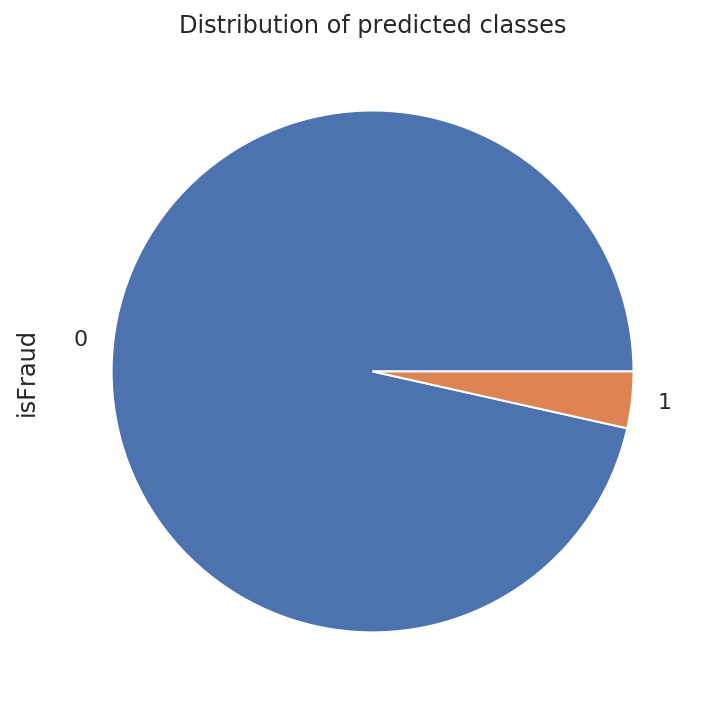
\includegraphics[width=0.5\textwidth]{figures/class_distribution.png}
    \end{center}
	\caption{Predicted classes distribution - data are highly imbalanced.}
	\label{fig:classes}
\end{figure}


\section{Method proposal}

% TODO: len kratko, co navrhujeme - feature selection na nejaky model pomocou nejakeho prirodou inspirovaneho algoritmu
% TODO: mozeno spomenut oversampling/undersampling


% usage of nature inspired algorithm proved to optimize feature selection much better than baseline well-known methods and overperforms  using power of nature inspired algorithms to address the problem of a lot of anonymized features available in existing datasets. Combination of machine learning and nature inspired algorithms proved to be the wa

% Proper data analysis in combination with training machine learning models can help to prevent frauds. Problem of choosing correct features without knowing their meaning with goal to improve detection performance can be seen as optimization problem. Nature inspired algorithms are known to be very powerful for optimization problems.





\section{Preparation}



% TODO: spomenut preprocessing, co sme robili a co z toho vzislo
% TODO: spomenut transformery, one hot, a filter
% TODO: kolko bol finalny pocet features
% TODO: len kratko spomenut ze preco sme sa rozhodli pouzit aky model - decision tree

\section{Experiments}

% TODO: ake experiemnty sme spravili
% TODO: tabulka porovnania algoritmov
% TODO: learning along the way with consequences - napr undersampling/oversampling atd.

\section{Conclusion}

% TODO: zhrnutie vysledkov, mozne vylepsenia a uskalia nasho pristupu

\bibliographystyle{splncs04}
\bibliography{references}

\end{document}
